%% Thinking Forth
%% Copyright (C) 2004 Leo Brodie
%% Initial transcription by Ed Beroset
%% 
%% test harness
%% pdflatex harness

\newif\ifpdf
\ifx\pdfoutput\undefined
  \pdffalse % we are not running PDFLaTeX
\else
  \pdfoutput=1 % we are running PDFLaTeX
  \pdftrue
\fi

\def\tfoptions{6.14x9.21,2004,tip,tipno,leo,isbn}
\def\tflang{american}
\def\isbn{0-9764587-0-5}
\def\linkcolor{blue}
\def\printing{Punchy Printing}
\def\tfversion{2.0-pre1}

\def\pagecount{81}


\ifpdf
\documentclass[10pt,\tflang,pdftex]{book}
\else
\documentclass[10pt,\tflang,dvips]{book}
\fi

\usepackage[T1]{fontenc}
\usepackage[latin1]{inputenc}
\usepackage{graphics}
\usepackage{babel}
\usepackage{geometry}
\usepackage{pst-all}
\usepackage{fancyvrb}
\usepackage[\tfoptions]{tf}

%% Cover creation howto:
%% back | spine | front + border
%% spine = pages*0.0041in
%% border: 0.25in

\newdimen\pwidth
\newdimen\pheight
\newdimen\oldpwidth
\newdimen\twidth
\newdimen\evenmargin
\newdimen\oddmargin
\oldpwidth\paperwidth
\twidth\textwidth
\oddmargin1in
\advance\oddmargin\evensidemargin
\advance\evenmargin\paperwidth
\advance\evenmargin-\twidth
\advance\evenmargin-\oddmargin
\newdimen\spine
\spine0.5\pthick
\spine\pagecount\spine
\pwidth2\paperwidth
\advance\pwidth\spine
\advance\pwidth2\cborder
\pheight\paperheight
\advance\pheight2\cborder

\geometry{verbose,paperwidth=\pwidth,paperheight=\pheight,tmargin=0in,%
bmargin=0in,lmargin=0in,rmargin=0in,headheight=0pt,headsep=0pt,%
footskip=0pt}

% for pdflatex
\ifpdf
\DeclareGraphicsExtensions{.pdf,.png,.jpg}
\else
\DeclareGraphicsExtensions{.eps}
\fi

\makeatletter
\advance\pheight-2\cborder
\parindent0pt
\begin{document}
\pagestyle{empty}
\centerline{\psframebox*[fillcolor=black,framesep=\cborder]{\noindent
\hbox{\white
\begin{minipage}{\oldpwidth}
\advance\leftskip\oddmargin
\vbox to\pheight{\vspace{0.5in}
\begin{minipage}{\twidth}%
\parindent2.5em\sf
%% Alternative back page, written by Bernd Paysan
%% you'll find the original back page at version 1.3 in the CVS repository

\noindent
\textbf{Thinking \Forth{}} is a book about the philosophy of problem
solving and programming style, applied to the unique programming
language `\Forth{}.' Published first in 1984, it could be among the
timeless classics of computer books, such as \person{Fred Brook}'s
\emph{The Mythical Man-Month} and \person{Donald Knuth}'s \emph{The
Art of Computer Programming}.

Many software engineering principles discussed here have been
rediscovered in eXtreme Programming, including (re)factoring,
modularity, bottom-up and incremental design.  Here you'll find all of
those and more, described in \person{Leo Brodie}'s down-to-earth,
humorous style, with illustrations, code examples, practical real life
applications, illustrative cartoons, and interviews with \Forth{}'s
inventor, \person{Charles H. Moore} as well as other Forth thinkers.

If you program in \Forth{}, this is a must-read book.  If you don't,
the fundamental concepts are universal: \textbf{Thinking \Forth{}} is
meant for anyone interested in writing software to solve problems.
The concepts go beyond \Forth{}, but the \emph{simple beauty} of
\Forth{} throws those concepts into stark relief.

So flip open the book, and read all about the philosophy of Forth,
analysis, decomposition, problem solving, style and conventions,
factoring, handling data, and minimizing control structures.  But be
prepared: you may not be able to put it down.

\medskip
This book has been scanned, OCR'd, typeset in \LaTeX{}, and brought
back to print (and your monitor) by a collaborative effort under a Creative
Commons license.

\medskip\blackline{0pt}\medskip
%%if you want Leo's picture here, uncommend this
\ifleo
\makeatletter
\setbox\@tempboxa\hbox{
\includegraphics{leobrodie}}
\rightmargin\wd\@tempboxa
\@tempdima\ht\@tempboxa
\advance\@tempdima-\ht\strutbox
\advance\rightmargin1em
\advance\textwidth-\rightmargin
\makeatother
\noindent\begin{tabular}{@{}p{\textwidth}@{\hspace{1em}}l@{}}
\parindent2.5em
\fi
\textbf{\person{Leo Brodie}} is a writer, programmer, consultant,
teacher, and world-renowned authority on \Forth. He was a technical
writer for \Forth{} Inc., and has been an independent consultant
(since 1982) for such clients as IBM, NCR, and Lockheed. He is also
the author of \emph{``Starting \Forth''} (Prentice-Hall, 1981).
\ifleo
& \makeatletter
\smash{\lower\@tempdima\hbox{
\includegraphics{leobrodie}}}
\makeatother \\
\end{tabular}
\fi
\end{minipage}
\vss
\psframebox*[fillcolor=white,framesep=.125in]{
\includegraphics{isbn}}
\vspace*{0.5in}}
\end{minipage}
\vline
\begin{minipage}{\spine}
\ifspineup
\expandafter\rotateleft
\else
\expandafter\rotateright
\fi
{\vbox to \spine{\vss\hbox to \pheight{%
    \fontfamily{phv}\selectfont
    \noindent\hspace{0.5in}%
    \Huge\bfseries\person{Leo Brodie}\hss
    \HUGE\slshape THINKING FORTH\/\hspace{0.5in}%
}\vss}}
\end{minipage}
\vline
\begin{minipage}{\oldpwidth}
\vbox to\pheight{\vspace{0.5in}
    \fontfamily{phv}\selectfont
  \vbox{\hrule \@height 3pt
  \HUGE
    \vspace*{0.2ex}\hbox to \textwidth{\hspace{\evenmargin}\bfseries Leo Brodie\hss}\vspace*{0.2ex}
    \hrule \@height 3pt}
  \vspace*{100pt}
%%if you want the thinker on the cover, use that:
\ifthinker
  \smash{\lower4.8in\hbox to\oldpwidth{\hss
  \smash{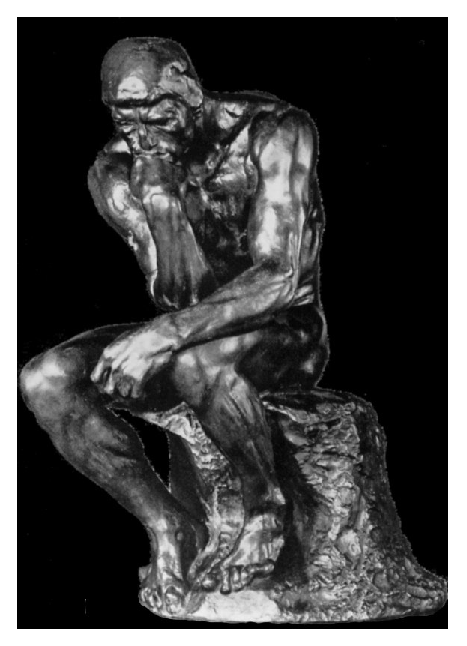
\includegraphics{rodin_thinker}}\hspace{0.125in}}}
\fi
  \hbox{\hspace{\evenmargin}
  \begin{minipage}{\twidth}
    \parindent\z@\hyphenpenalty 10000\raggedright
    {\THUGE\bfseries\slshape THINKING FORTH\\[1em]}
    \Huge A Language \\ and Philosophy \\ for Solving Problems
  \end{minipage}}
   \vfill
  \hbox{\hspace{\evenmargin}
  \begin{minipage}{\twidth}
     \Large\noindent Includes interviews with \Forth{}'s inventor,
\person{Charles H. Moore}, and other \Forth{} thinkers
  \end{minipage}}
\vspace{0.5in}}
\end{minipage}}}}


\end{document}
